% !TeX root = er.tex

\chapter{Kinématique d'un Manipulateur Robotique}\label{ch.kinematics}
\index{kinématique}

Notre présentation s'est concentrée sur les robots mobiles. La plupart des robots éducatifs sont des robots mobiles et vous avez peut-être déjà rencontré des robots mobiles commerciaux tels que des aspirateurs robotisés. Vous n'avez probablement pas rencontré de \emph{manipulateurs robotiques}, mais vous avez vu des images d'usines qui assemblent des circuits électroniques ou qui soudent des framed de voitures (Fig.~\ref{fig.assemblyline}). La différence la plus importante entre les robots mobiles et les robots fixes est l'environnement dans lequel ils travaillent. Un robot mobile se déplace dans un environnement comportant des obstacles et un sol irrégulier, de sorte que l'environnement n'est pas entièrement connu à l'avance. Un aspirateur robotisé ne vous demande pas de lui fournir un plan de votre appartement avec l'emplacement de chaque meuble, ni de le reprogrammer chaque fois que vous déplacez un canapé. Au lieu de cela, le robot détecte de manière autonome la disposition de l'appartement : les pièces et la position des meubles. Si les cartes et l'odométrie sont utiles pour déplacer un robot vers une position approximative, des capteurs doivent être utilisés pour localiser précisément le robot dans son environnement.

Un manipulateur robotique dans une usine est fixé à un sol en béton stable et sa construction est robuste : l'émission répétée des mêmes commandes déplacera le manipulateur exactement à la même position. Dans ce chapitre, nous présentons des algorithmes pour la cinématique des manipulateurs : comment les commandes données à un manipulateur et le mouvement du robot sont liés. La présentation se fera en termes de bras avec deux liens dans un plan dont les articulations peuvent tourner.

La cinématique comporte deux tâches complémentaires :
\begin{itemize}
\item \textit{Cinématique avant} (Sect.\ref{s.forward-kinematics}) : Compte tenu d'une séquence de commandes, quelle est la position finale du bras robotique ?
\item \textit{cinématique inverse} (Sect.~\ref{s.inverse-kinematics}) : Etant donné la position souhaitée du bras robotique, quelle séquence de commandes l'amènera à cette position ?
\end{itemize}

La cinématique avant est relativement facile à calculer, car le calcul du changement de position résultant du déplacement de chaque articulation fait appel à une simple trigonométrie. S'il y a plus d'une liaison, la position finale est calculée en effectuant les calculs pour une articulation après l'autre. La cinématique inverse est très difficile, car on part d'une position souhaitée et on doit chercher une séquence de commandes pour atteindre cette position. Un problème de cinématique inverse peut avoir une solution, plusieurs solutions ou même aucune solution.

Les calculs cinématiques sont effectués en termes de cadres de coordonnées. Un cadre est attaché à chaque articulation du manipulateur et le mouvement est décrit comme des transformations d'un cadre à un autre par des rotations et des translations. La transformation des cadres de coordonnées en deux dimensions est présentée dans les sections~\ref{s.rotations}--\ref{s.rotate-translate}. La plupart des robots manipulateurs sont tridimensionnels. Le traitement mathématique des mouvements en 3D dépasse le cadre de ce livre, mais nous espérons vous inciter à étudier ce sujet en vous présentant un aperçu des rotations en 3D dans les sections~\ref{s.three}--\ref{s.advanced-three}.

\section{Cinématique de l'avant}\label{s.forward-kinematics}

Nous développons la cinématique d'un bras robotique bidimensionnel avec deux liens, deux articulations et un \emph{effecteur final}\index{effecteur final} tel qu'une pince, une soudeuse ou un pulvérisateur de peinture (Fig.~\ref{fig.forward-kinematics}). La première articulation peut tourner, mais elle est montée sur une base fixée à une table ou au sol. La liaison $l_1$ relie cette articulation à une deuxième articulation qui peut se déplacer et tourner ; une deuxième liaison $l_2$ relie cette articulation à l'effecteur fixe.

Un système de coordonnées à deux dimensions est attribué avec la première articulation à $(0,0)$. Les longueurs des deux liens sont $l_1$ et $l_2$. Faites pivoter la première articulation de $\alpha$ pour déplacer l'extrémité de la première liaison avec la deuxième articulation à $(x',y')$. Faites maintenant pivoter la deuxième articulation de $\beta$. Quelles sont les coordonnées $(x,y)$ de l'extrémité du bras, en fonction des deux constantes $l_1,l_2$ et des deux paramètres $\alpha,\beta$ ?

\begin{figure}
\begin{center}
% Forward kinematics
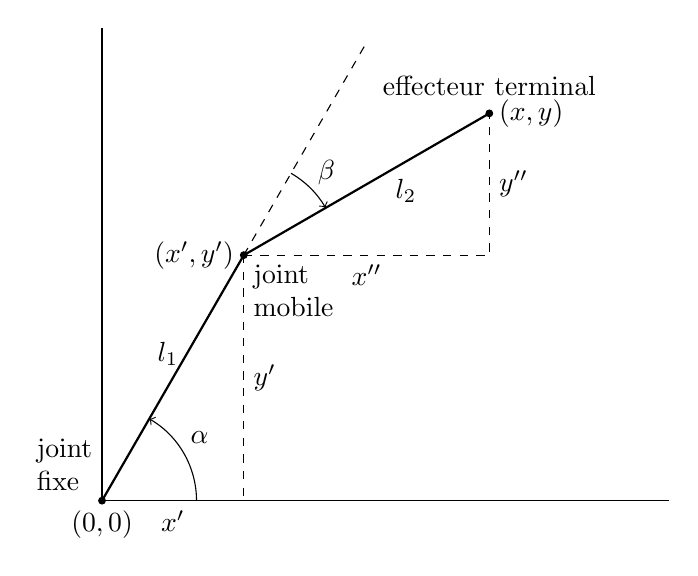
\begin{tikzpicture}[scale=1.2,align=left]
\draw (0,0) coordinate (origin) -- (6,0);
\draw (origin) -- (0,5);
\draw[thick] (origin) -- node[left,xshift=2mm,yshift=3mm] {$l_1$} ++(60:3) coordinate (prime) -- node[below,xshift=5mm,yshift=2mm] {$l_2$} ++(30:3) coordinate (point);
\path (origin) -- ++(60:3) -- ++(30:1) coordinate (angle);
\draw[dashed] (60:3) -- ++(60:2.6);
\draw[->] (1,0) arc (0:60:1) node[midway,xshift=2mm,yshift=2mm] {$\alpha$};
\draw[<-] (angle) arc (30:60:1) node[midway,xshift=2mm,yshift=2mm] {$\beta$};
\draw[fill] (origin) circle [radius=1pt] node[below] {$(0,0)$};
\draw[fill] (prime) circle [radius=1pt] node[left] {$(x',y')$};
\draw[fill] (point) circle [radius=1pt] node[right] {$(x,y)$};
\node[above,yshift=1mm] at (point) {\p{effecteur terminal}};
\node[above left] at (origin) {\p{joint}\\\p{fixe}};
\node[below right] at (prime) {\p{joint}\\\p{mobile}};
\draw[dashed] (prime) |- (origin);
\draw[dashed] (prime) -| (point);
\path (origin) -- node[below] {$x'$} (prime |- origin);
\path (prime |- origin) -- node[right] {$y'$} (prime);
\path (prime) -- node[below] {$x''$} (prime -| point);
\path (prime -| point) -- node[right] {$y''$} (point);
\end{tikzpicture}
\end{center}
\caption{Cinématique avant d'un bras à deux articulations}\label{fig.forward-kinematics}
\end{figure}

Projeter $(x',y')$ sur les axes $x$- et $y$- ; par trigonométrie ses coordonnées sont :
\begin{eqnarray*}
x' &=& l_1 \cos \alpha\\
y' &=& l_1 \sin \alpha\,.
\end{eqnarray*}
Prenons maintenant $(x',y')$ comme origine d'un nouveau système de coordonnées et projetons $(x,y)$ sur ses axes pour obtenir $(x'',y'')$. La position de l'effecteur dans le nouveau système de coordonnées est la suivante :
\begin{eqnarray*}
x'' &=& l_2 \cos (\alpha+\beta)\\
y'' &=& l_2 \sin (\alpha+\beta)\,.
\end{eqnarray*}
Dans la figure~\ref{fig.forward-kinematics}, $\beta$ est négatif (rotation dans le sens des aiguilles d'une montre), de sorte que $\alpha+\beta$ est l'angle entre le deuxième maillon et la ligne parallèle à l'axe $x$.

En combinant les résultats, on obtient
\begin{eqnarray*}
x &=& l_1 \cos \alpha + l_2 \cos(\alpha + \beta)\\
y &=& l_1 \sin \alpha + l_2 \sin(\alpha + \beta)\,.
\end{eqnarray*}

\noindent\textbf{Exemple} Soit $l_1 = l_2 = 1$, $\alpha = 60^{\circ}$, $\beta = -30^{\circ}$. Then:
\begin{eqnarray*}
x &=& 1\cdot\cos 60 + 1\cdot\cos(60-30) = \frac{1}{2} + \frac{\sqrt{3}}{2} = \frac{1+\sqrt{3}}{2}\\
y &=& 1\cdot\sin 60 + 1\cdot\sin(60-30) = \frac{\sqrt{3}}{2} + \frac{1}{2} = \frac{1+\sqrt{3}}{2}\,.
\end{eqnarray*}
Vérifions si ce résultat a un sens. La figure~\ref{fig.kinematics-triangle} montre un triangle formé par l'ajout d'une ligne entre $(0,0)$ et $(x,y)$. Le complément de l'angle $\beta$ est $180-30=150$ et le triangle est isocèle puisque les deux côtés sont $1$, donc les autres angles du triangle sont égaux et leurs valeurs sont $(180-150)/2=15$. L'angle que forme la nouvelle droite avec l'axe $x$ est $60-15=45$, ce qui est compatible avec $x=y$.

\begin{figure}
\begin{center}
% Angles of the triangle
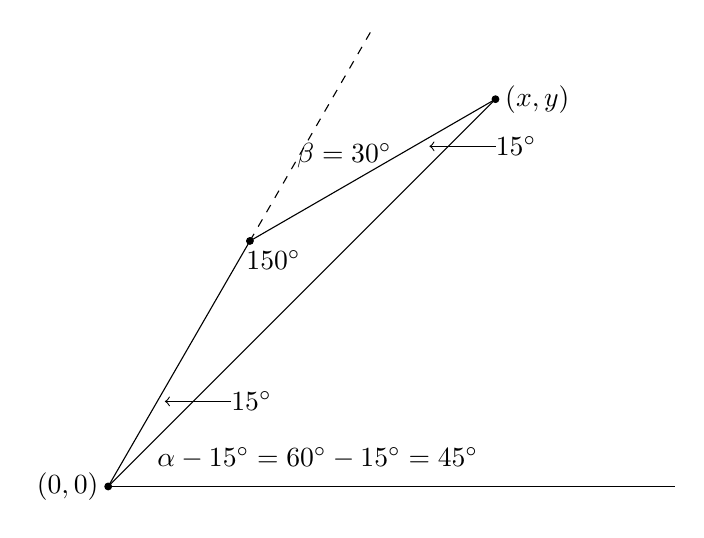
\begin{tikzpicture}[scale=1.2]
\draw (0,0) coordinate (origin) node[left] {$(0,0)$} -- (6,0);
\draw (origin) -- ++(60:3) coordinate (prime) -- ++(30:3) coordinate (point);
\path (origin) -- ++(60:3) -- ++(30:1) coordinate (angle);
\draw (origin) -- (point) node[right] {$(x,y)$};
\draw[dashed] (60:3) -- ++(60:2.6);
\draw[fill] (origin) circle [radius=1pt];
\draw[fill] (prime) circle [radius=1pt];
\draw[fill] (point) circle [radius=1pt];
\node[above,xshift=12mm,yshift=8mm] at (prime) {$\beta=30^{\circ}$};
\node[below,xshift=3mm,yshift=0mm] at (prime) {$150^{\circ}$};
\draw[->] (13mm,9mm) -- node[right,xshift=3mm] {$15^{\circ}$} (6mm,9mm);
\draw[->] (41mm,36mm) -- node[right,xshift=3mm] {$15^{\circ}$} (34mm,36mm);
\node[above right,xshift=5mm,yshift=1mm] at (origin) {$\alpha-15^{\circ}=60^{\circ}-15^{\circ}=45^{\circ}$};
\end{tikzpicture}
\end{center}
\caption{Calcul des angles}\label{fig.kinematics-triangle}
\end{figure}

\begin{framed}
\act{Cinématique vers l'avant}{kinématique vers l'avant}
\begin{itemize}
\item Programmez votre robot de manière à ce qu'il suive la trajectoire du bras de la Fig.~\ref{fig.forward-kinematics} : tournez à gauche $60^{\circ}$, avancez d'une unité ($1$m ou une autre distance convenable), tournez à droite $30^{\circ}$, avancez d'une unité.
\item Mesurer les distances $x$- et $y$- du robot par rapport à l'origine et les comparer aux valeurs calculées par les équations de la cinématique d'avancement.
\end{itemize}
\end{framed}

\section{Cinématique inverse}\label{s.inverse-kinematics}

L'anneau gris de la Fig.~\ref{fig.workspace} montre le \emph{workspace}\index{workspace} du bras à deux bras, l'ensemble des positions que l'effecteur peut atteindre (nous supposons que $l_2<l_1$). (Nous supposons que $l_2<l_1$.) L'espace de travail est circulairement symétrique puisque nous supposons qu'il n'y a pas de limites à la rotation des articulations sur un cercle complet entre $-180^{\circ}$ et $180^{\circ}$. Tout point tel que $a$ sur la circonférence du cercle extérieur est la position la plus éloignée du bras par rapport à l'origine ; elle est obtenue lorsque les deux maillons sont alignés de manière à ce que la longueur du bras soit $l_1+l_2$. Les positions les plus proches de l'origine dans l'espace de travail sont des points comme $b$ sur la circonférence du cercle intérieur ; elles sont obtenues lorsque le deuxième maillon est replié sur le premier maillon, ce qui donne une longueur de $l_1-l_2$. Une autre position atteignable $c$ est indiquée ; il existe \emph{deux} configurations (rotations des articulations) qui permettent au bras d'être positionné à $c$.

\begin{figure}
\begin{center}
% Workspace of two-level arm
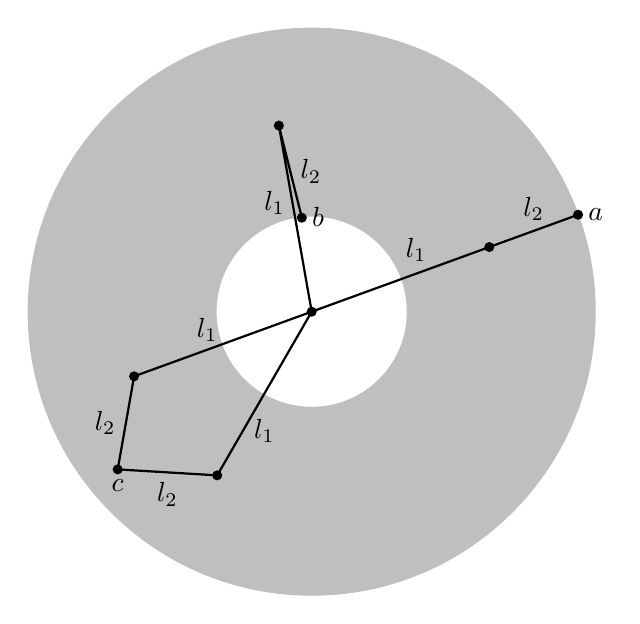
\begin{tikzpicture}[scale=.8]
% Circles
\draw[fill,gray!50] (0,0) coordinate (origin) circle[radius=45mm];
\draw[fill,white] (origin) circle[radius=15mm];
\draw[fill] (origin) circle [radius=2pt];
% First position
\draw[thick] (origin) -- node[above,xshift=2mm,yshift=1mm] {$l_1$} ++(20:30mm) -- node[above] {$l_2$} ++(20:15mm)  node[right] {$a$};
\draw[fill] (20:30mm) circle [radius=2pt];
\draw[fill] (20:45mm) circle [radius=2pt];
% Second position
\draw[thick] (origin) -- node[left,xshift=0mm,yshift=2mm] {$l_1$} ++(100:30mm) -- node[right] {$l_2$} ++(284:15mm)  node[right] {$b$};
\draw[fill] (100:30mm) circle [radius=2pt];
\draw[fill] (96:15mm) circle [radius=2pt];
% Third position
\draw[thick] (origin) -- node[above,xshift=-2mm,yshift=-1mm] {$l_1$} ++(200:30mm) coordinate (mid1) -- node[left] {$l_2$} ++(260:15mm) coordinate (endtwo) node[below] {$c$};
\draw[thick] (origin) -- node[below,,xshift=0mm,yshift=-2mm] {$l_1$} ++(240:30mm) coordinate (mid2) -- node[below] {$l_2$} (endtwo);
\draw[fill] (mid1) circle [radius=2pt];
\draw[fill] (mid2) circle [radius=2pt];
\draw[fill] (endtwo) circle [radius=2pt];
\end{tikzpicture}
\end{center}
\caption{Espace de travail d'un bras à deux leviers}\label{fig.workspace}
\end{figure}

Sous l'hypothèse que $l_2<l_1$, aucune séquence de rotations ne peut positionner l'extrémité du bras plus près de l'origine que $l_1-l_2$ et aucune position à une distance supérieure à $l_1+l_2$ de l'origine n'est accessible. La figure nous apprend qu'un problème de cinématique inverse, c'est-à-dire la recherche de commandes pour atteindre un point spécifié, peut avoir zéro, une ou plusieurs solutions.

Le calcul de la cinématique inverse utilise la \emph{loi des cosinus} (Fig.~\ref{fig.cosines}) :
\[
a^2 + b^2 - 2ab \cos \theta = c^2\,.
\]
Dans un triangle rectangle $\cos 90^{\circ} = 0$ et la loi se réduit au théorème de Pythagore.

\begin{figure}
\begin{center}
% Law of cosines
\begin{tikzpicture}
\draw (0,0) coordinate (origin) --  node[below] {$c$} (6,0) coordinate (two);
\draw (origin) -- node[left] {$a$} ++(60:3) coordinate (one) -- node[above] {$b$} (two);
\node[below,xshift=1mm,yshift=-2mm] at (one) {$\theta$};
\end{tikzpicture}
\end{center}
\caption{Loi des cosinus}\label{fig.cosines}
\end{figure}

Supposons maintenant que l'on nous donne un point $(x,y)$ et que nous voulions des valeurs pour $\alpha,\beta$ (s'il en existe) qui amèneront le bras à ce point. Figure~\ref{fig.inverse-kinematics} similaire à la Fig.~\ref{fig.kinematics-triangle} sauf que les valeurs spécifiques sont remplacées par des angles et des longueurs arbitraires.

Par le théorème de Pythagore, $r=\sqrt{x^2 + y^2}$.
\begin{figure}
\begin{center}
% Inverse kinematics
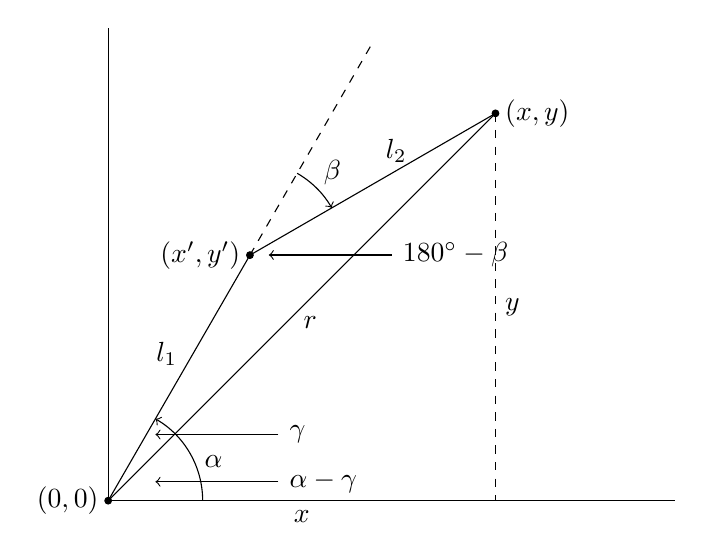
\begin{tikzpicture}[scale=1.2]
\draw (0,0) coordinate (origin) -- (6,0);
\draw (origin) -- (0,5);
\draw (origin) -- node[left,xshift=1mm,yshift=3mm] {$l_1$} ++(60:3) coordinate (prime) -- node[below,xshift=3mm,yshift=7mm] {$l_2$} ++(30:3) coordinate (point);
\draw[dashed] (point) -- node[right] {$y$} (point |- origin);
\draw (origin) -- node[below] {$x$} (origin -| point);
\path (origin) -- ++(60:3) -- ++(30:1) coordinate (angle);
\draw[dashed] (60:3) -- ++(60:2.6);
\draw (origin) -- node[right,xshift=-1mm,yshift=-2mm] {$r$} (point);
\draw[->] (1,0) arc (0:60:1) node[midway,xshift=3mm,yshift=-1mm] {$\alpha$};
\draw[<-] (angle) arc (30:60:1) node[midway,xshift=2mm,yshift=2mm] {$\beta$};
\draw[fill] (origin) circle [radius=1pt] node[left] {$(0,0)$};
\draw[fill] (prime) circle [radius=1pt] node[left] {$(x',y')$};
\draw[fill] (point) circle [radius=1pt] node[right] {$(x,y)$};

\draw[->] (30mm,26mm) -- node[right,xshift=8mm] {$180^{\circ}-\beta$} (17mm,26mm);
\draw[->] (18mm,7mm) -- node[right,xshift=8mm] {$\gamma$} (5mm,7mm);
\draw[->] (18mm,2mm) -- node[right,xshift=8mm] {$\alpha-\gamma$} (5mm,2mm);
\end{tikzpicture}
\end{center}
\caption{Cinématique inverse d'un bras à deux articulations}\label{fig.inverse-kinematics}
\end{figure}

La loi des cosinus donne
\[
l_1^2 + l_2^2 - 2l_1 l_2 \cos(180^\circ-\beta) = r^2\,,
\]
qui peut être résolu pour $\beta$:
\begin{eqnarray*}
\cos(180^\circ-\beta) &=& \frac{l_1^2 + l_2^2 - r^2}{2l_1 l_2}\\
\beta &=& 180^\circ-\cos^{-1}\left(\frac{l_1^2 + l_2^2 - r^2}{2l_1 l_2}\right)\,.
\end{eqnarray*}
Pour obtenir $\gamma$ puis $\alpha$, utiliser la loi des cosinus avec $\gamma$ comme angle central :
\[
\cos\gamma = \frac{l_1^2 +r^2 - l_2^2}{2l_1 r}\,.
\]
Du triangle rectangle formé par $(x,y)$ on a :
\begin{eqnarray*}
\tan(\alpha - \gamma) &=& \frac{y}{x}\\
\alpha &=& \tan^{-1} \frac{y}{x} + \gamma\,,
\end{eqnarray*}
donc :
\[
\alpha = \tan^{-1} \frac{y}{x} + \cos^{-1}\left(\frac{l_1^2 +r^2 - l_2^2}{2l_1 r}\right)\,.
\]

\noindent\textbf{Exemple} Supposons à nouveau que $l_1 = l_2 = 1$ et que l'effecteur se trouve au point calculé à partir de la cinématique avant :
\[
(x,y) = \left(\frac{1+\sqrt{3}}{2},\frac{1+\sqrt{3}}{2}\right)\,.
\]
Tout d'abord, calculez $r^2$ :
\[
r^2 = x^2+y^2 = \left( \frac{1+\sqrt{3}}{2}\right)^2 + \left( \frac{1+\sqrt{3}}{2}\right)^2 = 2+\sqrt{3}\,,
\]
et l'utiliser dans le calcul de $\beta$ :
\begin{eqnarray*}
\beta &=& 180^{\circ} - \cos^{-1} \left(\frac{1^2 + 1^2 - (2+\sqrt{3})}{2\cdot 1\cdot 1}\right)\\
&=& 180^{\circ} - \cos^{-1}\left(-\frac{\sqrt{3}}{2}\right)\\
&=& 180^{\circ} \pm 150^{\circ}\\
&=& \pm 30^{\circ}\,,
\end{eqnarray*}
puisque $330^{\circ}=-30^{\circ} \!\!\!\pmod{360^\circ}$. Il y a deux solutions car il y a deux façons de déplacer le bras vers $(x,y)$.

Calculons ensuite $\gamma$ :
\begin{equation}
\gamma = \cos^{-1}\left(\frac{1^2 + r^2 - 1^2}{2\cdot 1 \cdot r}\right) = \cos^{-1}\left(\frac{r}{2}\right)= \cos^{-1}\left(\frac{\sqrt{2+\sqrt{3}}}{2}\right) = \pm 15^{\circ}\,.\label{eq.cos15}
\end{equation}
Le cosinus inverse peut être obtenu numériquement sur une calculatrice ou algébriquement comme indiqué dans l'Annexe~\ref{a.cosine}.

Puisque $x=y$, le calcul de $\alpha$ est facile :
\[\alpha = \tan^{-1}\frac{y}{x} + \gamma = \tan^{-1}1 + \gamma = 45^{\circ} \pm 15^{\circ} = 60^{\circ} \;\textrm{or}\; 30^{\circ}\,.
\]
La solution $\alpha=60^{\circ},\beta=-30^{\circ}$ correspond à la rotation des articulations de la Fig.~\ref{fig.forward-kinematics}, tandis que la solution $\alpha=30^{\circ},\beta=30^{\circ}$ correspond à une rotation des deux articulations de $30^{\circ}$ dans le sens inverse des aiguilles d'une montre.

Dans ce cas simple, il est possible de résoudre l'équation de la cinématique directe pour obtenir les formules de la cinématique inverse. En général, cela n'est pas possible, c'est pourquoi des solutions numériques approximatives sont utilisées.

\begin{framed}
\act{Cinématique inverse}{kinématique inverse}
\begin{itemize}
\item Utilisez les formules de la cinématique inverse pour programmer votre robot afin qu'il se déplace vers une coordonnée donnée.
\item Mesurer les distances $x$- et $y$- du robot par rapport à l'origine et les comparer aux coordonnées spécifiées.
\item Si l'ordinateur de votre robot n'a pas la capacité de calculer les formules, calculez-les hors ligne et entrez ensuite les commandes au robot.
\end{itemize}
\end{framed}

%%%%%%%%%%%%%%%%%%%%%%%%%%%%%%%%%%%%%%%%%%%%%%%%%%%%%%%%%%%

\section{Rotations}\label{s.rotations}
\index{rotation}

Le mouvement d'un manipulateur robotique est décrit en termes de \emph{cadres de coordonnées}\index{cadres de coordonnées}. Trois cadres sont associés au bras de la Fig.~\ref{fig.forward-kinematics} : un cadre est associé à l'articulation à l'origine (que nous supposons fixée à une table ou au sol), un deuxième cadre est associé à l'articulation entre les deux liens, et un troisième cadre est associé à l'effecteur à l'extrémité du deuxième lien.

Dans cette section, nous décrivons comment le mouvement de rotation d'un bras robotique peut être modélisé mathématiquement à l'aide de \emph{matrices de rotation}. Les liens des bras robotiques introduisent des \emph{translations} : la deuxième articulation est décalée d'une distance linéaire de $l_1$ par rapport à la première articulation, et l'effecteur est décalé d'une distance linéaire de $l_2$ par rapport à la deuxième articulation. Le traitement mathématique des translations utilise une extension des matrices de rotation appelée \emph{transformations homogènes}.

Les rotations peuvent prêter à confusion car une matrice de rotation peut avoir trois interprétations qui sont décrites dans les sous-sections suivantes : rotation d'un vecteur, rotation d'un cadre de coordonnées et transformation d'un vecteur d'un cadre de coordonnées à un autre.

\subsection{Rotation d'un vecteur}
\index{rotation!vecteur@d'un vecteur}

Considérons un vecteur avec des coordonnées cartésiennes $(x,y)$ et des coordonnées polaires $(r,\phi)$ (Fig.~\ref{fig.one-vector}). On fait maintenant pivoter le vecteur d'un angle $\theta$ (Fig.~\ref{fig.rotated-vector}). Ses coordonnées polaires sont $(r,\phi+\theta)$. Quelles sont ses coordonnées cartésiennes ?

\begin{figure}
\begin{minipage}{.48\textwidth}
\begin{tikzpicture}[scale=1.2]
\draw (0,0) coordinate (origin) -- (4,0);
\draw (origin) -- (0,3);
\path[->] (origin) -- ++(30:3.5) coordinate (point);
\draw[->] (origin) -- node[above] {$r$} ++(30:3.46);
\draw[fill] (point) circle [radius=1pt];
\draw (point) -- node[right] {$y$} (point |- origin);
\draw (origin) -- node[below,xshift=2mm] {$x$} (point |- origin);
\draw (1,0) arc (0:30:1) node[midway,xshift=3mm] {$\phi$};
\draw[fill] (origin) circle [radius=1pt];
\end{tikzpicture}
\caption{Un vecteur}\label{fig.one-vector}
\end{minipage}
\hspace{\fill}
\begin{minipage}{.48\textwidth}
\begin{tikzpicture}[scale=1.2]
\draw (0,0) coordinate (origin) -- (4,0);
\draw (origin) -- (0,3);
\path[->] (origin) -- ++(60:3.5) coordinate (point);
\draw[->] (origin) -- node[above] {$r$} ++(60:3.46);
\draw[fill] (point) circle [radius=1pt];
\draw (point) -- node[right] {$y'$} (point |- origin);
\draw (origin) -- node[below,xshift=2mm] {$x'$} (point |- origin);
\draw (1,0) arc (0:60:1);
\node at (1.2,.7) {$\phi+\theta$};
\draw[fill] (origin) circle [radius=1pt];
\end{tikzpicture}
\caption{Le vecteur tourné par $\theta$}\label{fig.rotated-vector}
\end{minipage}
\end{figure}

En utilisant les identités trigonométriques pour la somme de deux angles et la conversion de $(r,\phi)$ en $(x,y)$ nous avons :
\begin{eqnarray*}
x' &=& r\cos(\phi+\theta)\\
&=&r\cos\phi\cos\theta - r\sin\phi\sin\theta\\
&=&(r\cos\phi)\cos\theta - (r\sin\phi)\sin\theta\\
&=&x\cos\theta - y\sin\theta\,,\\
\\
y' &=& r\sin(\phi+\theta)\\
&=&r\sin\phi\cos\theta + r\cos\phi\sin\theta\\
&=&(r\sin\phi)\cos\theta + (r\cos\phi)\sin\theta\\
&=&y\cos\theta + x\sin\theta\\
&=&x\sin\theta + y\cos\theta\,.\\
\end{eqnarray*}
Ces équations peuvent être exprimées comme la multiplication d'une matrice appelée \emph{matrice de rotation}\index{matrice de rotation!bidimensionnelle} et d'un vecteur :
\[
\spacearray
\left[\begin{array}{c}x'\\y'\end{array}\right]=
\left[\begin{array}{cc}\cos\theta&-\sin\theta\\\sin\theta&\cos\theta\end{array}\right]
\left[\begin{array}{c}x\\y\end{array}\right]\,.
\]

\medskip

\noindent\textbf{Exemple} Soit $p$ le point situé à l'extrémité d'un vecteur de longueur $r=1$ qui forme un angle de $\phi=30^{\circ}$ avec l'axe positif $x$. Les coordonnées cartésiennes de $p$ sont $\left(\frac{\sqrt{3}}{2},\,\frac{1}{2}\right)$. Supposons que le vecteur subisse une rotation de $\theta=30^{\circ}$. Quelles sont les nouvelles coordonnées cartésiennes de $p$ ? En utilisant la multiplication des matrices :
\[
\spacearray
\left[\begin{array}{c}x'\\y'\end{array}\right]\;=\;
\left[\begin{array}{cc}\frac{\sqrt{3}}{2}&-\frac{1}{2}\\\frac{1}{2}&\frac{\sqrt{3}}{2}\end{array}\right]
\left[\begin{array}{c}\frac{\sqrt{3}}{2}\\\frac{1}{2}\end{array}\right]\;=\;
\left[\begin{array}{c}\frac{1}{2}\\\frac{\sqrt{3}}{2}\end{array}\right]\,.
\]
Le résultat est logique car la rotation d'un vecteur dont l'angle avec l'axe $x$ est $30^{\circ}$ par $30^{\circ}$ devrait donner un vecteur dont l'angle avec l'axe $x$ est $60^{\circ}$.

Supposons que le vecteur subisse une rotation supplémentaire de $30^{\circ}$ ; ses nouvelles coordonnées sont :
\begin{equation}\label{eq.rotate1}
\spacearray
\left[\begin{array}{cc}\frac{\sqrt{3}}{2}&-\frac{1}{2}\\\frac{1}{2}&\frac{\sqrt{3}}{2}\end{array}\right]\;\;
\left(\left[\begin{array}{cc}\frac{\sqrt{3}}{2}&-\frac{1}{2}\\\frac{1}{2}&\frac{\sqrt{3}}{2}\end{array}\right]
\left[\begin{array}{c}\frac{\sqrt{3}}{2}\\\frac{1}{2}\end{array}\right]\right)\;=\;
\left[\begin{array}{cc}\frac{\sqrt{3}}{2}&-\frac{1}{2}\\\frac{1}{2}&\frac{\sqrt{3}}{2}\end{array}\right]
\left[\begin{array}{c}\frac{1}{2}\\\frac{\sqrt{3}}{2}\end{array}\right]\;=\;
\left[\begin{array}{c}0\\1\end{array}\right]\,.
\end{equation}
Ce résultat est également logique. La rotation d'un vecteur dont l'angle est de $30^{\circ}$ deux fois par $30^{\circ}$ (pour un total de $60^\circ$) devrait donner $90^{\circ}$. Le cosinus de $90^{\circ}$ est $0$ et le sinus de $90^{\circ}$ est $1$.

La multiplication matricielle étant associative, la multiplication peut également être effectuée comme suit :
\begin{equation}\label{eq.rotate2}
\spacearray
\left(\left[\begin{array}{cc}\frac{\sqrt{3}}{2}&-\frac{1}{2}\\\frac{1}{2}&\frac{\sqrt{3}}{2}\end{array}\right]
\left[\begin{array}{cc}\frac{\sqrt{3}}{2}&-\frac{1}{2}\\\frac{1}{2}&\frac{\sqrt{3}}{2}\end{array}\right]\right)\;\;
\left[\begin{array}{c}\frac{\sqrt{3}}{2}\\\frac{1}{2}\end{array}\right]\,.
\end{equation}

\begin{framed}
\act{Matrices de rotation}{Matrice de rotation}
\begin{itemize}
\item Démontrer l'associativité de la multiplication matricielle en montrant que la multiplication dans Eq.~\ref{eq.rotate2} donne le même résultat que la multiplication dans Eq.~\ref{eq.rotate1}.
\item Calculer la matrice pour une rotation de $-30^{\circ}$ et montrer que la multiplication de cette matrice par la matrice pour une rotation de $30^{\circ}$ donne la matrice pour une rotation de $0^{\circ}$.
\item Cette multiplication est-elle commutative ?
\item La multiplication des matrices de rotation à deux dimensions est-elle commutative ?
\end{itemize}
\end{framed}

\subsection{Rotation d'un cadre de coordonnées}
\index{rotation!coordonnée@d'un repère de coordonnées}

Réinterprétons les figures~\ref{fig.one-vector}--\ref{fig.rotated-vector}. La figure~\ref{fig.one-frame} montre un cadre de coordonnées (bleu) défini par deux vecteurs unitaires orthogonaux :
\[
\vec{x}= \left[\begin{array}{c}1\\0\end{array}\right]\,,\;\;
\vec{y}= \left[\begin{array}{c}0\\1\end{array}\right]\,.
\]
La figure \ref{fig.frame-rotated} montre le \emph{bâtiment de coordonnées} tourné de $\theta$ degrés (rouge). Les nouveaux vecteurs unitaires $\vec{x'}$ et $\vec{y'}$ peuvent être obtenus en les multipliant par la matrice de rotation dérivée ci-dessus :
\begin{eqnarray*}
\vec{x'}&=&
\left[\spacearray\begin{array}{cc}\cos\theta&-\sin\theta\\\sin\theta&\cos\theta\end{array}\right]
\left[\spacearray\begin{array}{c}1\\0\end{array}\right]=
\left[\spacearray\begin{array}{l}\cos \theta\\\sin\theta\;\;\:\end{array}\right]\\
\,\\
\vec{y'}&=&
\left[\spacearray\begin{array}{cc}\cos\theta&-\sin\theta\\\sin\theta&\cos\theta\end{array}\right]
\left[\spacearray\begin{array}{c}0\\1\end{array}\right]=
\left[\spacearray\begin{array}{l}-\sin \theta\\\cos\theta\end{array}\right]\,.
\end{eqnarray*}

\begin{figure}
\begin{minipage}{.48\textwidth}
\begin{tikzpicture}[scale=1.2]
\draw (0,0) coordinate (origin) -- (3.4,0);
\draw (origin) -- (0,2.8);
\draw[->,thick,blue] (0,0) -- node[below] {$\vec{x}$} (2,0);
\draw[->,thick,blue] (0,0) -- node[left] {$\vec{y}$} (0,2);
\end{tikzpicture}
\caption{Cadre de coordonnées original (bleu)}\label{fig.one-frame}
\end{minipage}
\hspace{\fill}
\begin{minipage}{.48\textwidth}
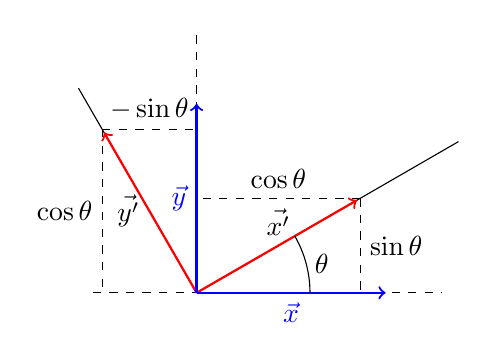
\begin{tikzpicture}[scale=1.2]
\begin{scope}[rotate=30]
\draw (0,0) coordinate (origin) -- (3.2,0);
\draw (origin) -- (0,2.5);
\path (0,0) -- node[above] {$\vec{x'}$} (2,0) coordinate (xprime);
\path (0,0) -- node[left] {$\vec{y'}$} (0,2) coordinate (yprime);
\draw[->,thick,red] (0,0) -- (1.96,0);
\draw[->,thick,red] (0,0) -- (0,1.96);
\end{scope}
\draw[dashed] (-1.1,0) -- (origin) -- (2.6,0);
\draw[dashed] (origin) -- (0,2.8);
\draw[->,thick,blue] (0,0) -- node[below] {$\vec{x}$} (2,0);
\draw[->,thick,blue] (0,0) -- node[left] {$\vec{y}$} (0,2);
\draw[dashed] (xprime) -- node[right] {$\sin \theta$} (xprime |- origin);
\draw[dashed] (xprime) -- node[above] {$\cos \theta$} (origin |- xprime);
\draw[dashed] (yprime) -- node[left] {$\cos \theta$} (yprime |- origin);
\draw[dashed] (yprime) -- node[above] {$-\sin \theta$} (origin |- yprime);
\draw (1.2,0) arc (0:30:1.2) node[midway,xshift=2mm,yshift=0mm] {$\theta$};
\end{tikzpicture}
\caption{Nouveau cadre de coordonnées (rouge) obtenu en faisant pivoter le cadre de coordonnées original (bleu) de $\theta$}\label{fig.frame-rotated}
\end{minipage}
\end{figure}

\medskip

\noindent\textbf{Exemple} Pour les vecteurs unitaires de la Fig.~\ref{fig.one-frame} et une rotation de $30^\circ$:
\begin{eqnarray*}
\vec{x'}&=&\left[\spacearray\begin{array}{cc}\frac{\sqrt{3}}{2}&-\frac{1}{2}\\\frac{1}{2}&\frac{\sqrt{3}}{2}\end{array}\right]
\left[\spacearray\begin{array}{c}1\\0\end{array}\right]=
\left[\spacearray\begin{array}{c}\frac{\sqrt{3}}{2}\\\frac{1}{2}\end{array}\right]\\
\,\\
\vec{y'}&=&\left[\spacearray\begin{array}{cc}\frac{\sqrt{3}}{2}&-\frac{1}{2}\\\frac{1}{2}&\frac{\sqrt{3}}{2}\end{array}\right]
\left[\spacearray\begin{array}{c}0\\1\end{array}\right]=
\left[\spacearray\begin{array}{c}-\frac{1}{2}\\\frac{\sqrt{3}}{2}\end{array}\right]\,.
\end{eqnarray*}

\subsection{Transformation d'un vecteur d'un repère à un autre}
\index{rotation!transformation d'un vecteur d'un repère de coordonnées à un autre}

L'origine d'un repère de coordonnées $b$ (bleu) représente l'articulation d'un effecteur tel qu'une soudeuse et le point $p$ est l'extrémité de la soudeuse (\ref{fig.frameb}). Par convention en robotique, le cadre de coordonnées d'une entité est désigné par un exposant " pré ".\footnote{La convention est d'utiliser des lettres majuscules à la fois pour le cadre et les coordonnées, mais nous utilisons des minuscules pour plus de clarté.}  Dans le framed $b$, le point $\bp$ a des coordonnées polaires $(r,\phi)$ et des coordonnées cartésiennes $(\bx,\by)$ reliées par les formules trigonométriques habituelles :
\[
\bp = (\bx,\by) = (r\cos\phi,\, r\sin\phi)\,.
\]

\begin{figure}
\begin{minipage}{.48\textwidth}
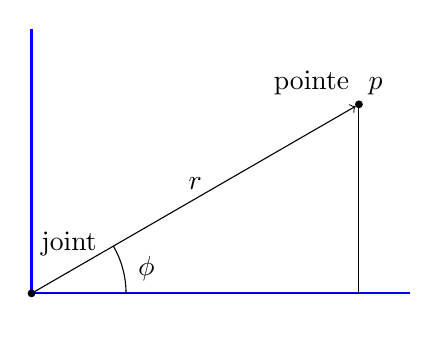
\begin{tikzpicture}[scale=1.2]
\draw[thick,blue] (0,0) coordinate (origin) -- (4,0);
\draw[thick,blue] (origin) -- (0,2.8);
\path (origin) -- node[above] {$r$} ++(30:4) coordinate (point) node[above right] {$p$};
\draw[->] (origin) -- ++(30:3.96);
\draw[fill] (point) circle [radius=1pt] node[above left] {\p{pointe}};
\draw (point) -- node[right] {$\by$} (point |- origin);
\draw (origin) -- node[below,xshift=2mm] {$\bx$} (point |- origin);
\draw (1,0) arc (0:30:1) node[midway,xshift=3mm] {$\phi$};
\draw[fill] (origin) circle [radius=1pt] node[above right,yshift=10pt] {\p{joint}};
\end{tikzpicture}
\caption{Point $p$ à l'extrémité d'un effecteur dans le repère de coordonnées $b$ (bleu)}\label{fig.frameb}
\end{minipage}
\hspace{\fill}
\begin{minipage}{.48\textwidth}
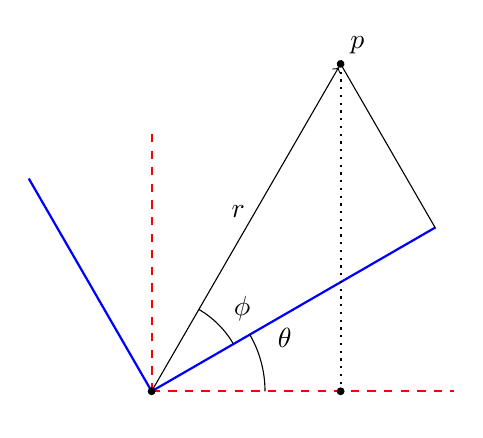
\begin{tikzpicture}[scale=1.2]
\begin{scope}[rotate=30]
\draw[thick,blue] (0,0) coordinate (origin) -- node[black,below,xshift=12mm,yshift=6mm] {$\bx$} (3.47,0);
\draw[thick,blue] (origin) -- (0,2.6);
\path (origin) -- node[above,xshift=-1mm] {$r$} ++(30:4) coordinate (point) node[above right] {$p$};
\draw[->] (origin) -- ++(30:3.96);
\draw[fill] (point) circle [radius=1pt];
\draw (point) -- node[right] {$\by$} (point |- origin);
\draw (1,0) arc (0:30:1) node[midway,xshift=3mm,yshift=2mm] {$\phi$};
\end{scope}
\draw[thick,dashed,red] (origin) -- (3.2,0);
\draw[thick,dashed,red] (origin) -- (0,2.8);
\draw[thick,dotted] (point) -- node[right] {$\ay$} (point |- origin);
\draw[fill] (point |- origin) circle [radius=1pt];
\path[dashed] (origin) -- node[below,xshift=2mm] {$\ax$} (point |- origin);
\draw (1.2,0) arc (0:30:1.2) node[midway,xshift=3mm,yshift=3mm] {$\theta$};
\draw[fill] (origin) circle [radius=1pt];
\end{tikzpicture}
\caption{Point $p$ dans les cadres de coordonnées $a$ (rouge) et $b$ (bleu)}\label{fig.framea}
\end{minipage}
\end{figure}

Supposons que l'articulation (\emph{avec son cadre de coordonnées}) subisse une rotation de l'angle $\theta$. Les coordonnées du point par rapport à $b$ restent les mêmes, mais le cadre de coordonnées a été déplacé. Nous posons donc la question suivante : quelles sont les coordonnées $\ap=(\ax,\ay)$ du point dans le cadre de coordonnées avant qu'il n'ait été déplacé ? Dans la figure \ref{fig.framea}, le cadre original $b$ est représenté tourné vers une nouvelle position (et toujours en bleu), tandis que le cadre de coordonnées $a$ se trouve dans l'ancienne position de $b$ et est représenté par des lignes pointillées rouges. Dans la section précédente, nous avons demandé comment transformer un cadre de coordonnées en un autre ; ici, nous demandons comment transformer les coordonnées d'un point dans un cadre en ses coordonnées dans un autre cadre.

En ce qui concerne le bras robotique, nous connaissons $(\bx,\by)$, les coordonnées de l'extrémité de l'effecteur par rapport au framed de l'effecteur, et nous demandons maintenant ses coordonnées $\ap=(\ax,\ay)$ par rapport à la base fixe. Ceci est important car si nous connaissons $\ap$, nous pouvons calculer la distance et l'angle entre l'extrémité de la soudeuse et les parties de la voiture qu'elle doit maintenant souder.

Nous pouvons répéter le calcul utilisé pour la rotation d'un vecteur :
\begin{eqnarray*}
\ax &=& r\cos(\phi+\theta)\\
&=&r\cos\phi\cos\theta - r\sin\phi\sin\theta\\
&=&\bx\cos\theta - \by\sin\theta\,,\\
\\
\ay &=& r\sin(\phi+\theta)\\
&=&r\sin\phi\cos\theta + r\cos\phi\sin\theta\\
&=&\bx\sin\theta + \by\cos\theta\,,\\
\end{eqnarray*}
pour obtenir la matrice de rotation :
\begin{equation}
\spacearray
\left[\begin{array}{c}\ax\\\ay\end{array}\right]=
\left[\begin{array}{cc}\cos\theta&-\sin\theta\\\sin\theta&\cos\theta\end{array}\right]
\left[\begin{array}{c}\bx\\\by\end{array}\right]\,.\label{eq.frame-to-frame}
\end{equation}
La matrice est appelée matrice de rotation \emph{de} l'image $b$ \emph{à} l'image $a$ et est notée $\leftidx{^a_b}{R}{}$. La prémultiplication du point $\bp$ dans le repère $b$ par la matrice de rotation donne à $\ap$ ses coordonnées dans le repère $a$ :
\[
\ap = \leftidx{^a_b}{R}{} \; \bp\,.
\]

\medskip

\noindent\textbf{Exemple} Soit $\bp$ le point du repère $b$ situé à l'extrémité d'un vecteur de longueur $r=1$ qui forme un angle de $\phi=30^{\circ}$ avec l'axe positif $x$. Les coordonnées de $\bp$ sont $\left(\frac{\sqrt{3}}{2},\,\frac{1}{2}\right)$. Supposons que le cadre de coordonnées $b$ (ainsi que le point $p$) subisse une rotation de $\theta=30^{\circ}$ pour obtenir le cadre de coordonnées $a$. Quelles sont les coordonnées de $\ap$ ? En utilisant l'Eq.~\ref{eq.frame-to-frame} :
\[
\spacearray
\ap=
\left[\begin{array}{c}\ax\\\ay\end{array}\right]\;=\;
\left[\begin{array}{cc}\frac{\sqrt{3}}{2}&-\frac{1}{2}\\\frac{1}{2}&\frac{\sqrt{3}}{2}\end{array}\right]
\left[\begin{array}{c}\frac{\sqrt{3}}{2}\\\frac{1}{2}\end{array}\right]\;=\;
\left[\begin{array}{c}\frac{1}{2}\\\frac{\sqrt{3}}{2}\end{array}\right]\,.
\]
Si le cadre $a$ subit une rotation de $30^{\circ}$, on obtient les coordonnées du point dans un troisième cadre $a1$. Pré-multiplier $\ap$ par la matrice de rotation pour $30^{\circ}$ pour obtenir $\aprimep$ :
\[
\spacearray
\aprimep = \left[\begin{array}{cc}\frac{\sqrt{3}}{2}&-\frac{1}{2}\\\frac{1}{2}&\frac{\sqrt{3}}{2}\end{array}\right]\;\;
\left(\left[\begin{array}{cc}\frac{\sqrt{3}}{2}&-\frac{1}{2}\\\frac{1}{2}&\frac{\sqrt{3}}{2}\end{array}\right]
\left[\begin{array}{c}\frac{\sqrt{3}}{2}\\\frac{1}{2}\end{array}\right]\right)\;=\;
\left[\begin{array}{cc}\frac{\sqrt{3}}{2}&-\frac{1}{2}\\\frac{1}{2}&\frac{\sqrt{3}}{2}\end{array}\right]
\left[\begin{array}{c}\frac{1}{2}\\\frac{\sqrt{3}}{2}\end{array}\right]\;=\;
\left[\begin{array}{c}0\\1\end{array}\right]\,.
\]
Le produit des deux matrices de rotation :
\[
\spacearray
\left[\begin{array}{cc}\frac{\sqrt{3}}{2}&-\frac{1}{2}\\\frac{1}{2}&\frac{\sqrt{3}}{2}\end{array}\right]
\left[\begin{array}{cc}\frac{\sqrt{3}}{2}&-\frac{1}{2}\\\frac{1}{2}&\frac{\sqrt{3}}{2}\end{array}\right]=
\left[\begin{array}{cc}\frac{1}{2}&-\frac{\sqrt{3}}{2}\\\frac{\sqrt{3}}{2}&\frac{1}{2}\end{array}\right]
\]
donne la matrice de rotation pour faire pivoter le cadre de coordonnées original $b$ de $60^{\circ}$ :
\[
\spacearray
\left[\begin{array}{cc}\frac{1}{2}&-\frac{\sqrt{3}}{2}\\\frac{\sqrt{3}}{2}&\frac{1}{2}\end{array}\right]
\left[\begin{array}{c}\frac{\sqrt{3}}{2}\\\frac{1}{2}\end{array}\right]\;=\;
\left[\begin{array}{c}0\\1\end{array}\right]\,.
\]
Étant donné une séquence de rotations, la prémultiplication de leurs matrices de rotation donne la matrice de rotation pour la rotation équivalente à la somme des rotations individuelles.

\section{Rotation et translation d'un cadre de coordonnées}\label{s.rotate-translate}

Les articulations des manipulateurs robotiques sont reliées par des liens, de sorte que les systèmes de coordonnées sont liés non seulement par des rotations, mais aussi par des translations. Le point $p$ de la Fig.~\ref{fig.before-rotate} représente un point dans le repère de coordonnées (rouge) $b$, mais par rapport au repère de coordonnées (bleu en pointillés) $a$, le repère $b$ subit une rotation de l'angle $\theta$ et son origine est translatée de $\Delta x$ et $\Delta y$. Si l'on connaît $\bp=(\bx,\by)$, les coordonnées du point dans le repère $b$, quelles sont ses coordonnées $\ap=(\ax,\ay)$ dans le repère $a$ ?

\begin{figure}
\begin{center}
\begin{tikzpicture}[scale=1.2]
\begin{scope}[yshift=1cm,xshift=3cm,rotate around={30:(0,0)}]
\draw[thick,red] (0,0) coordinate (origin) -- node[black,near end,xshift=8mm,yshift=-2mm] {\p{cadre b}} (4,0);
\draw[thick,red] (origin) -- (0,3);
\path (origin) -- node[above,xshift=-1mm] {$r$} ++(30:4) coordinate (point) node[above right] {$p$};
\draw[->] (origin) -- ++(30:3.96);
\draw[fill] (point) circle [radius=1pt];
\draw (point) -- node[right] {$\by$} (point |- origin);
\path (origin) -- node[below,xshift=5mm,yshift=2mm] {$\bx$} (point |- origin);
\draw (1,0) arc (0:30:1) node[midway,xshift=3mm,yshift=2mm] {$\phi$};
\end{scope}
\draw[dashed,thick,blue] (0,0) coordinate (origina) -- node[black,below,midway,yshift=-1mm] {\p{cadre a}} (6,0);
\draw[dashed,thick,blue] (origina) -- (0,3);
\draw[->] (origina) -- ($ (origina) ! .985 ! (point) $);
\draw[dashed] (origin) -- (point |- origin);
\draw (4.5,1) arc (0:30:1.45) node[midway,xshift=2mm] {$\theta$};
\draw[dotted,thick] (origin) -- (origin |- origina) node [right,midway] {$\Delta y$};
\draw[dotted,thick] (origin) -- (origina |- origin) node [below,midway] {$\Delta x$};
\draw[fill] (origin) circle [radius=1pt];
\draw[fill] (origina) circle [radius=1pt];
\end{tikzpicture}
\caption{La frame $b$ subit une rotation et une translation vers la frame $a$}\label{fig.before-rotate}
\end{center}
\end{figure}
Pour effectuer ce calcul, nous définissons un repère intermédiaire (vert) $a1$ qui a la même origine que $b$ et la même orientation que $a$ (Fig.~\ref{fig.after-rotate}). Quelles sont les coordonnées $\aprimep=(\aprimex,\aprimey)$ du point dans le cadre $a1$ ? Il s'agit simplement de la rotation par $\theta$ que nous avons effectuée précédemment :
\[
\spacearray
\aprimep=\left[\begin{array}{c}\aprimex\\\aprimey\end{array}\right]=
\left[\begin{array}{cc}\cos\theta&-\sin\theta\\\sin\theta&\cos\theta\end{array}\right]
\left[\begin{array}{c}\bx\\\by\end{array}\right]\,.
\]
Maintenant que nous avons les coordonnées du point dans $a1$, il est facile d'obtenir les coordonnées dans le framed $a$ en ajoutant les décalages de la translation. Sous forme de matrice :
\[
\spacearray
\ap=\left[\begin{array}{c}\ax\\\ay\end{array}\right]=
\left[\begin{array}{c}\aprimex\\\aprimey\end{array}\right]\,+\,
\left[\begin{array}{c}\Delta x\\\Delta y\end{array}\right]\,.
\]

\begin{figure}
\begin{center}
\begin{tikzpicture}[scale=1.2]
\begin{scope}[yshift=1cm,xshift=3cm,rotate around={30:(0,0)}]
\draw[thick,red] (0,0) coordinate (origin) -- node[black,near end,xshift=8mm,yshift=-2mm] {\p{cadre b}} (4,0);
\draw[thick,red] (origin) -- (0,3);
\path (origin) -- ++(30:4) coordinate (point) node[above right] {$p$};
\draw[->] (origin) -- ++(30:3.96);
\draw[fill] (point) circle [radius=1pt];
\draw (1,0) arc (0:30:1) node[midway,xshift=3mm,yshift=2mm] {$\phi$};
\end{scope}
\draw[thick,green!60!black] (origin) -- node[black,below,midway,xshift=4mm] {\p{cadre a1}} +(4,0);
\draw[thick,green!60!black] (origin) -- +(0,4);
\draw[dotted,thick] (point) -- node [right,midway] {$\aprimey$} (point |- origin);
\draw[dotted,thick] (point) -- node [above,midway] {$\aprimex$} (origin |- point);
\draw[dashed,thick,blue] (0,0) coordinate (origina) -- node[black,below,midway,yshift=-1mm] {\p{cadre a}} (6,0);
\draw[dashed,thick,blue] (origina) -- (0,3);
\draw[->] (origina) -- ($ (origina) ! .985 ! (point) $);
\draw (4.5,1) arc (0:30:1.45) node[midway,xshift=2mm] {$\theta$};
\draw[dotted,thick] (origin) -- (origin |- origina) node [right,midway] {$\Delta y$};
\draw[dotted,thick] (origin) -- (origina |- origin) node [below,midway] {$\Delta x$};
\draw[fill] (origin) circle [radius=1pt];
\draw[fill] (origina) circle [radius=1pt];
\end{tikzpicture}
\caption{Le cadre $b$ subit une rotation jusqu'au cadre $a1$, puis une translation jusqu'au cadre $a$}.\label{fig.after-rotate}
\end{center}
\end{figure}

\emph{transformations homogènes}\index{transformations homogènes} sont utilisées pour combiner une rotation et une translation en un seul opérateur. Le vecteur bidimensionnel donnant les coordonnées d'un point est étendu avec un troisième élément qui a une valeur fixe de $1$ :
\[
\spacearray
\left[\begin{array}{c}x\\y\\1\end{array}\right]\,.
\]
La matrice de rotation est étendue à une matrice $3 \times 3$ avec un $1$ dans le coin inférieur droit et des zéros ailleurs. Il est facile de vérifier que la multiplication d'un vecteur dans le cadre $b$ par la matrice de rotation donne le même vecteur qu'auparavant, à l'exception de l'élément $1$ supplémentaire :
\[
\spacearray
\left[\begin{array}{c}\leftidx{^{a1}}\!{x}{}\\\leftidx{^{a1}}\!{y}{}\\1\end{array}\right]\;=\;
\left[\begin{array}{ccc}\cos\theta&-\sin\theta&0\\\sin\theta&\cos\theta&0\\0&0&1\end{array}\right]
\left[\begin{array}{c}\bx\\\by\\1\end{array}\right]\,.
\]
Le résultat est les coordonnées du point dans le framed intermédiaire $a1$. Pour obtenir les coordonnées dans le cadre $a$, on multiplie par une matrice qui effectue la translation :
\[
\spacearray
\left[\begin{array}{c}\ax\\\ay\\1\end{array}\right]\;=\;
\left[\begin{array}{ccc}1&0&\Delta x\\0&1&\Delta y\\0&0&1\end{array}\right]
\left[\begin{array}{c}\leftidx{^{a1}}\!{x}{}\\\leftidx{^{a1}}\!{y}{}\\1\end{array}\right]\,.
\]
En multipliant les deux transformées, on obtient une seule transformée homogène qui peut effectuer à la fois la rotation et la translation :
\[
\spacearray
\left[\begin{array}{ccc}1&0&\Delta x\\0&1&\Delta y\\0&0&1\end{array}\right]
\left[\begin{array}{ccc}\cos\theta&-\sin\theta&0\\\sin\theta&\cos\theta&0\\0&0&1\end{array}\right]\;=\;
\left[\begin{array}{ccc}\cos\theta&-\sin\theta&\Delta x\\\sin\theta&\cos\theta&\Delta y\\0&0&1\end{array}\right]\,.
\]
\noindent\textbf{Exemple} Étendons l'exemple précédent en ajoutant une translation de $(3,1)$ à la rotation de $30^\circ$. La transformée homogène de la rotation suivie de la translation est :
\[
\spacearray
\left[\begin{array}{ccc}1&0&3\\0&1&1\\0&0&1\end{array}\right]
\left[\begin{array}{ccc}\frac{\sqrt{3}}{2}&-\frac{1}{2}&0\\\frac{1}{2}&\frac{\sqrt{3}}{2}&0\\0&0&1\end{array}\right]\;\;=
\left[\begin{array}{ccc}\frac{\sqrt{3}}{2}&-\frac{1}{2}&3\\\frac{1}{2}&\frac{\sqrt{3}}{2}&1\\0&0&1\end{array}\right]\,.
\]
Les coordonnées du point dans le cadre $a$ sont :
\[
\spacearray
\left[\begin{array}{c}\ax\\\ay\\1\end{array}\right]\;=\;
\left[\begin{array}{ccc}\frac{\sqrt{3}}{2}&-\frac{1}{2}&3\\\frac{1}{2}&\frac{\sqrt{3}}{2}&1\\0&0&1\end{array}\right]
\left[\begin{array}{c}\frac{\sqrt{3}}{2}\\\frac{1}{2}\\1\end{array}\right]\;=\;
\left[\begin{array}{c}\frac{1}{2}+3\\\frac{\sqrt{3}}{2}+1\\1\end{array}\right]\,.
\]

\begin{framed}
\act{transformations homogènes}{homogènes}
\begin{itemize}
\item Dessinez le diagramme d'une rotation de $-30^\circ$ suivie d'une translation de $(3,-1)$.
\item Calculer la transformée homogène.
\end{itemize}
\end{framed}

%%%%%%%%%%%%%%%%%%%%%%%%%%%%%%%%%%%%%%%%%%%%%%%%%%%%%%%%%%%

\section{Un goût de rotations tridimensionnelles}\label{s.three}
\index{rotation!tridimensionnelle}

Les concepts de transformation des coordonnées et de cinématique en trois dimensions sont les mêmes qu'en deux dimensions, mais les mathématiques sont plus complexes. En outre, beaucoup d'entre nous ont du mal à visualiser un mouvement tridimensionnel lorsque tout ce qui nous est montré est une représentation bidimensionnelle d'objets tridimensionnels. Dans cette section, nous donnerons un avant-goût de la robotique tridimensionnelle en examinant les rotations en trois dimensions.

\subsection{Rotations autour des trois axes}\label{s.rotation-notation}

Un repère de coordonnées bidimensionnel $x$-$y$ peut être considéré comme étant encadré dans un repère de coordonnées tridimensionnel en ajoutant un axe $z$ perpendiculaire aux axes $x$ et $y$. La figure \ref{fig.frame} montre une représentation bidimensionnelle du cadre tridimensionnel. L'axe $x$ est tracé à gauche et à droite sur le papier et l'axe $y$ est tracé de haut en bas. La ligne diagonale représente l'axe $z$ qui est perpendiculaire aux deux autres axes. Le cadre de coordonnées "standard" $x$-$y$-$z$ a les directions positives de ses axes définies par la règle de la main droite (voir ci-dessous). Les directions positives sont \textit{droite} pour l'axe $x$, \textit{haut} pour l'axe $y$ et \textit{sortie} (du papier vers l'observateur) pour l'axe $z$. 

\begin{figure}
\begin{center}
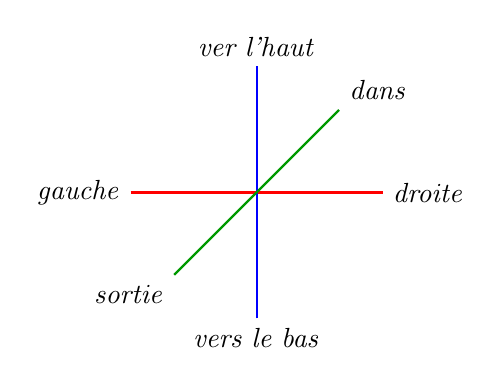
\begin{tikzpicture}[scale=.8]
\draw[thick,red] (-2,0,0) node [black,left] {\textit{gauche}} -- (2,0,0) node [black,right] {\textit{droite}};
\draw[thick,blue] (0,-2,0) node [black,below] {\textit{vers le bas}} -- (0,2,0) node [black,above] {\textit{ver l'haut}};
\draw[thick,green!60!black] (0,0,-3.4) node [black,above right] {\textit{dans}} -- (0,0,3.4) node [black,below left] {\textit{sortie}};
\end{tikzpicture}
\caption{Cadre de coordonnées tridimensionnelles}\label{fig.frame}
\end{center}
\end{figure}

Faire pivoter le cadre de coordonnées dans le sens inverse des aiguilles d'une montre autour de l'axe $z$, de sorte que l'axe $z$ reste inchangé (Figs.~\ref{fig.standard-axis1}-\ref{fig.rotatez}). La nouvelle orientation du framed est (\textit{ver l'haut}, \textit{gauche}, \textit{sortie}). Considérons maintenant une rotation de $90^irc$ autour de l'axe $x$ (Figs.~\ref{fig.standard-axis2}--\ref{fig.rotatex}). L'axe $y$ sort alors du papier et l'axe $z$ tombe sur le papier, ce qui donne l'orientation (\textit{droite}, \textit{sortie}, \textit{ver le bas}). Enfin, considérons une rotation de $90^\circ$ autour de l'axe $y$ (Figs.~\ref{fig.standard-axis3}--\ref{fig.rotatey}). L'axe $x$ "tombe" dans le papier et l'axe $z$ "tombe" sur le papier. La nouvelle position du framed est (\textit{dans}, \textit{ver l'haut}, \textit{right}).

\begin{figure}
\begin{minipage}{.48\textwidth}
\begin{tikzpicture}[scale=1.2]
\draw[thick,red,->] (0,0,0) -- (2,0,0) node [black,right] {$x$};
\draw [thick,blue,->] (0,0,0) -- (0,2,0) node [black,above] {$y$};
\draw [thick,green!60!black,->] (0,0,0) -- (0,0,2) node [black,below left] {$z$};
\draw[->] (.5,0,1) arc [start angle=0, end angle=270, radius=3.5mm];
\end{tikzpicture}
\caption{$x$-$y$-$z$ cadre de coordonnées}\label{fig.standard-axis1}
\end{minipage}
\hspace{\fill}
\begin{minipage}{.48\textwidth}
\begin{tikzpicture}[scale=1.2]
\draw [thick,blue,->] (0,0,0) -- (-2,0,0) node [black,left] {$y$};
\draw [thick,red,->] (0,0,0) -- (0,2,0) node [black,above] {$x$};
\draw [thick,green!60!black,->] (0,0,0) -- (0,0,2) node [black,below left] {$z$};
\end{tikzpicture}
\caption{$x$-$y$-$z$ cadre de coordonnées après rotation de $90^\circ$ autour de l'axe $z$}\label{fig.rotatez}
\end{minipage}
\end{figure}


\begin{figure}
\begin{minipage}{.48\textwidth}
\begin{tikzpicture}[scale=1.2]
\draw [thick,red,->] (0,0,0) -- (2,0,0) node [black,right] {$x$};
\draw [thick,blue,->] (0,0,0) -- (0,2,0) node [black,above] {$y$};
\draw [thick,green!60!black,->] (0,0,0) -- (0,0,2) node [black,below left] {$z$};
\draw[->] (1,.1,0) arc [start angle=0, end angle=270, radius=3.5mm];
\end{tikzpicture}
\caption{cadre de coordonnées $x$-$y$-$z$}\label{fig.standard-axis2}
\end{minipage}
\hspace{\fill}
\begin{minipage}{.48\textwidth}
\begin{tikzpicture}[baseline=-4em,scale=1.2]
\draw [thick,red,->] (0,0,0) -- (2,0,0) node [black,right] {$x$};
\draw [thick,green!60!black,->] (0,0,0) -- (0,-2,0) node [black,below] {$z$};
\draw [thick,blue,->] (0,0,0) -- (0,0,2) node [black,below left] {$y$};
\end{tikzpicture}
\caption{base de coordonnées $x$-$y$-$z$ après une rotation de $90^\circ$ autour de l'axe $x$}\label{fig.rotatex}
\end{minipage}
\end{figure}

\begin{figure}
\begin{minipage}{.48\textwidth}
\begin{tikzpicture}[scale=1.2]
\draw [thick,red,->] (0,0,0) -- (2,0,0) node [black,right] {$x$};
\draw [thick,blue,->] (0,0,0) -- (0,2,0) node [black,above] {$y$};
\draw [thick,green!60!black,->] (0,0,0) -- (0,0,2) node [black,below left] {$z$};
\draw[->] (.3,.8,0) arc [start angle=45, end angle=315, radius=3.5mm];
\end{tikzpicture}
\caption{cadre de coordonnées $x$-$y$-$z$}\label{fig.standard-axis3}
\end{minipage}
\hspace{\fill}
\begin{minipage}{.48\textwidth}
\begin{tikzpicture}[baseline=-3.8em,scale=1.2]
\draw [thick,green!60!black,->] (0,0,0) -- (2,0,0) node [black,right] {$z$};
\draw [thick,blue,->] (0,0,0) -- (0,2,0) node [black,above] {$y$};
\draw [thick,red,->] (0,0,0) -- (0,0,-2) node [black,above right] {$x$};
\end{tikzpicture}
\caption{cadre de coordonnées $x$-$y$-$z$ après une rotation de $90^\circ$ autour de l'axe $y$}\label{fig.rotatey}
\end{minipage}
\end{figure}

\subsection{La règle de la main droite}

Il y a deux orientations pour chaque axe, soit $2^3=8$ orientations au total. Ce qui compte, c'est l'orientation relative d'un axe par rapport aux deux autres ; par exemple, une fois que les axes $x$- et $y$- ont été choisis pour se situer dans le plan du papier, l'axe $z$ peut avoir sa direction positive pointant vers l'extérieur du papier ou vers l'intérieur du papier. Le choix doit être cohérent. La convention en physique et en mécanique est la \emph{règle de la main droite}\index{règle de la main droite}. Courbez les doigts de votre main droite de manière à ce qu'ils passent d'un axe à un autre. Votre pouce pointe maintenant dans la direction positive du troisième axe. Pour les axes familiers $x$- et $y$- sur le papier, recourbez vos doigts sur le chemin allant de l'axe $x$ à l'axe $y$. Ce faisant, votre pouce pointe vers l'extérieur du papier, ce qui est considéré comme la direction positive de l'axe $z$. La figure \ref{fig.right-hand-rule} montre le système de coordonnées de la main droite avec chacun des trois axes pointant \emph{hors du papier}. Selon la règle de la main droite, les trois rotations sont :
\begin{quote}
\normalsize
Rotation de x à y autour de z,\\
Rotation de y à z autour de x\\
Rotation de z à x autour de y.
\end{quote}

\begin{figure}
\begin{center}
\begin{tikzpicture}[scale=.85]
\draw [thick,red,->] (0,0,0) -- (2,0,0) node [black,right] {$x$};
\draw [thick,blue,->] (0,0,0) -- (0,2,0) node [black,above] {$y$};
\draw [thick,green!60!black,->] (0,0,0) -- (0,0,2) node [black,below left] {$z$};
\draw[->] (.5,0,1) arc [start angle=0, end angle=270, radius=3.5mm];
\end{tikzpicture}
\hspace{2em}
\begin{tikzpicture}[scale=.85]
\draw [thick,blue,->] (0,0,0) -- (2,0,0) node [black,right] {$y$};
\draw [thick,green!60!black,->] (0,0,0) -- (0,2,0) node [black,above] {$z$};
\draw [thick,red,->] (0,0,0) -- (0,0,2) node [black,below left] {$x$};
\draw[->] (.5,0,1) arc [start angle=0, end angle=270, radius=3.5mm];
\end{tikzpicture}
\hspace{2em}
\begin{tikzpicture}[scale=.85]
\draw [thick,green!60!black,->] (0,0,0) -- (2,0,0) node [black,right] {$z$};
\draw [thick,red,->] (0,0,0) -- (0,2,0) node [black,above] {$x$};
\draw [thick,blue,->] (0,0,0) -- (0,0,2) node [black,below left] {$y$};
\draw[->] (.5,0,1) arc [start angle=0, end angle=270, radius=3.5mm];
\end{tikzpicture}
\caption{La règle de droite}\label{fig.right-hand-rule}
\end{center}
\end{figure}

\subsection{Matrices pour les rotations tridimensionnelles}
\index{matrice!rotation!tridimensionnelle}

Une matrice de rotation tridimensionnelle est une matrice $3 fois 3$ car chaque point $p$ d'un framed a trois coordonnées $p_x,p_y,p_z$ qui doivent être déplacées. 
Commençons par une rotation de $\psi$ autour de l'axe $z$, suivie d'une rotation de $\theta$ autour de l'axe $y$ et enfin d'une rotation de $\phi$ autour de l'axe $x$. Pour la première rotation autour de l'axe $z$, les coordonnées $x$ et $y$ sont tournées comme en deux dimensions et la coordonnée $z$ reste inchangée. Par conséquent, la matrice est :
\[
\spacearray
R_{z(\psi)}=\left[\begin{array}{ccc}\cos\psi&-\sin\psi&0\\\sin\psi&\cos\psi&0\\0&0&1\end{array}\right]\,.
\]
Pour la rotation par $\theta$ autour de l'axe $y$, la coordonnée $y$ est inchangée et les coordonnées $z$ et $x$ sont transformées "comme si" elles étaient les coordonnées $x$ et $y$ d'une rotation autour de l'axe $z$ :
\[
\spacearray
R_{y(\theta)}=\left[\begin{array}{ccc}\cos\theta&0&\sin\theta\\0&1&0\\-\sin\theta&0&\cos\theta\\\end{array}\right]\,.
\]
Pour la rotation par $\phi$ autour de l'axe $x$, la coordonnée $x$ est inchangée et les coordonnées $y$ et $z$ sont transformées "comme si" elles étaient les coordonnées $x$ et $y$ d'une rotation autour de l'axe $z$ :
\[
\spacearray
R_{x(\phi)}=\left[\begin{array}{ccc}1&0&0\\0&\cos\phi&-\sin\phi\\0&\sin\phi&\cos\phi\\\end{array}\right]\,.
\]
Il peut sembler étrange que dans la matrice pour la rotation autour de l'axe $y$ les signes de la fonction sinus aient changé. Pour vous convaincre que la matrice pour cette rotation est correcte, redessinez le diagramme de la Fig.~\ref{fig.framea}, en remplaçant $z$ par $x$ et $x$ par $y$ et effectuez le calcul trigonométrique.

\subsection{Multiples rotations}

Il y a une mise en garde à propos de la composition des rotations : comme pour la multiplication matricielle, rotations tridimensionnelles \emph{ne pas} commuter. Démontrons-le à l'aide d'une simple séquence de deux rotations. Considérons une rotation de $90^\circ$ autour de l'axe $z$, suivie d'une rotation de $90^\circ$ autour de la (nouvelle position de) l'axe $x$ (Fig.~\ref{fig.non-commutative1}). Le résultat peut être exprimé par (\textit{up}, \textit{out}, \textit{droite}).
\begin{figure}
\begin{center}
\begin{tikzpicture}[scale=.85]
\draw [thick,red,->] (0,0,0) -- (2,0,0) node [black,right] {$x$};
\draw [thick,blue,->] (0,0,0) -- (0,2,0) node [black,above] {$y$};
\draw [thick,green!60!black,->] (0,0,0) -- (0,0,2) node [black,below left] {$z$};
\draw[->] (.5,0,1) arc [start angle=0, end angle=270, radius=3.5mm];
\end{tikzpicture}
\hspace{2em}
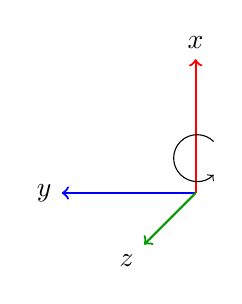
\begin{tikzpicture}[scale=.85]
\draw [thick,blue,->] (0,0,0) -- (-2,0,0) node [black,left] {$y$};
\draw [thick,red,->] (0,0,0) -- (0,2,0) node [black,above] {$x$};
\draw [thick,green!60!black,->] (0,0,0) -- (0,0,2) node [black,below left] {$z$};
\draw[->] (.5,1,.6) arc [start angle=45, end angle=315, radius=3.5mm];
\end{tikzpicture}
\hspace{2em}
\begin{tikzpicture}[scale=.85]
\draw [thick,green!60!black,->] (0,0,0) -- (2,0,0) node [black,right] {$z$};
\draw [thick,red,->] (0,0,0) -- (0,2,0) node [black,above] {$x$};
\draw [thick,blue,->] (0,0,0) -- (0,0,2) node [black,below left] {$y$};
\end{tikzpicture}
\caption{Rotation autour de l'axe $z$ suivie d'une rotation autour de l'axe $x$.}\label{fig.non-commutative1}
\end{center}
\end{figure}

Considérons maintenant l'opération commuée : une rotation de $90^\circ$ autour de l'axe $x$, suivie d'une rotation de $90^\circ$ autour de l'axe $z$ (Fig.~\ref{fig.non-commutative2}). Le résultat peut être exprimé comme (\textit{out}, \textit{gauche}, \textit{bas}), ce qui n'est pas la même chose que l'orientation précédente.

\begin{figure}
\begin{center}
\begin{tikzpicture}[scale=.85]
\draw [thick,red,->] (0,0,0) -- (2,0,0) node [black,right] {$x$};
\draw [thick,blue,->] (0,0,0) -- (0,2,0) node [black,above] {$y$};
\draw [thick,green!60!black,->] (0,0,0) -- (0,0,2) node [black,below left] {$z$};
\draw[->] (1.4,.1,0) arc [start angle=0, end angle=270, radius=3.5mm];
\end{tikzpicture}
\hspace{2em}
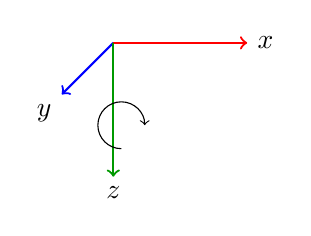
\begin{tikzpicture}[scale=.85,baseline=-3.1em]
\draw [thick,red,->] (0,0,0) -- (2,0,0) node [black,right] {$x$};
\draw [thick,blue,->] (0,0,0) -- (0,0,2) node [black,below left] {$y$};
\draw [thick,green!60!black,->] (0,0,0) -- (0,-2,0) node [black,below] {$z$};
\draw[<-] (.7,-1,.6) arc [start angle=0, end angle=270, radius=3.5mm];
\end{tikzpicture}
\hspace{2em}
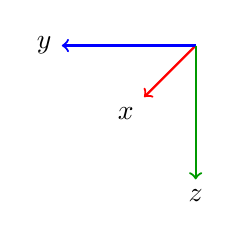
\begin{tikzpicture}[scale=.85,baseline=-3em]
\draw [thick,red,->] (0,0,0) -- (0,0,2) node [black,below left] {$x$};
\draw [thick,blue,->] (0,0,0) -- (-2,0,0) node [black,left] {$y$};
\draw [thick,green!60!black,->] (0,0,0) -- (0,-2,0) node [black,below] {$z$};
\end{tikzpicture}
\caption{Rotation autour de l'axe $x$ suivie d'une rotation autour de l'axe $z$}
\label{fig.non-commutative2}
\end{center}
\end{figure}

\subsection{angles d'Euler}
\index{angles d'Euler}

Une rotation arbitraire peut être obtenue par trois rotations individuelles autour des trois axes, de sorte que la matrice pour une rotation arbitraire peut être obtenue en multipliant les matrices pour chaque rotation individuelle. Les angles des rotations sont appelés \emph{angles d'Euler}. Les formules sont quelque peu complexes et peuvent être trouvées dans les références citées à la fin du chapitre. Nous démontrons ici les angles d'Euler à l'aide d'un exemple.

\smallskip

\noindent\textbf{Exemple} La figure~\ref{fig.euler} montre un cadre de coordonnées tourné séquentiellement $90^\circ$ autour de l'axe $z$, puis de l'axe $y$ et enfin de l'axe $x$. C'est ce qu'on appelle une rotation d'angle d'Euler $zyx$. L'orientation finale est (\textit{in}, \textit{up}, \textit{right}).

\begin{figure}
\begin{center}
\begin{tikzpicture}[scale=.7]
\draw [thick,red,->] (0,0,0) -- (2,0,0) node [black,right] {$x$};
\draw [thick,blue,->] (0,0,0) -- (0,2,0) node [black,above] {$y$};
\draw [thick,green!60!black,->] (0,0,0) -- (0,0,2) node [black,below left] {$z$};
\draw[->] (0,-.3,.1) arc [start angle=0, end angle=270, radius=3mm];
\end{tikzpicture}
\hspace{2em}
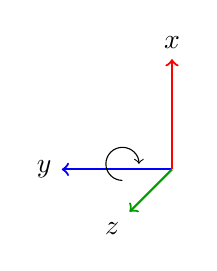
\begin{tikzpicture}[scale=.7]
\draw [thick,blue,->] (0,0,0) -- (-2,0,0) node [black,left] {$y$};
\draw [thick,red,->] (0,0,0) -- (0,2,0) node [black,above] {$x$};
\draw [thick,green!60!black,->] (0,0,0) -- (0,0,2) node [black,below left] {$z$};
\draw[<-] (-.6,.1,0) arc [start angle=0, end angle=270, radius=3mm];
\end{tikzpicture}
\hspace{2em}
\begin{tikzpicture}[scale=.7,baseline=-3em]
\draw [thick,green!60!black,->] (0,0,0) -- (0,2,0) node [black,above] {$z$};
\draw [thick,blue,->] (0,0,0) -- (-2,0,0) node [black,left] {$y$};
\draw [thick,red,->] (0,0,0) -- (0,0,-2.5) node [black,above right] {$x$};
\draw[<-] (.6,.2,-.5) arc [start angle=0, end angle=270, radius=3mm];
\end{tikzpicture}
\hspace{2em}
\begin{tikzpicture}[scale=.7,baseline=-3em]
\draw [thick,blue,->] (0,0,0) -- (0,2,0) node [black,above] {$y$};
\draw [thick,green!60!black,->] (0,0,0) -- (2,0,0) node [black,right] {$z$};
\draw [thick,red,->] (0,0,0) -- (0,0,-2.5) node [black,above right] {$x$};
\end{tikzpicture}
\caption{Angles d'Euler $zyx$ de $(90^\circ,90^\circ,90^\circ)$}\label{fig.euler}
\end{center}
\end{figure}

Considérons un manipulateur robotique composé d'une seule articulation qui peut tourner autour des trois axes. Une séquence de rotations est effectuée comme le montre la Fig.~\ref{fig.euler}. Considérons le point aux coordonnées $(1,1,1)$ par rapport à l'articulation (Fig.~\ref{fig.rotate3}). Après les rotations, quelles sont les coordonnées de ce point dans le framed original ?

\begin{figure}
\begin{minipage}{.48\textwidth}
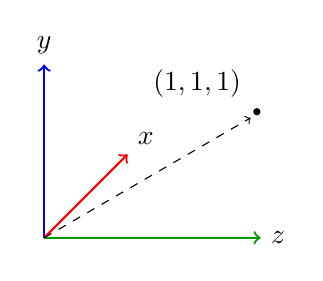
\begin{tikzpicture}[scale=1.1]
\draw [thick,blue,->] (0,0,0) -- (0,2,0) node [black,above] {$y$};
\draw [thick,green!60!black,->] (0,0,0) -- (2.5,0,0) node [black,right] {$z$};
\draw [thick,red,->] (0,0,0) -- (0,0,-2.5) node [black,above right] {$x$};
\draw[->,dashed] (0,0,0) -- (2,1,-1) node[above left,yshift=4pt] {$(1,1,1)$};
\draw[fill] (2,1,-1) circle [xshift=2pt,yshift=2pt,radius=1pt];
\end{tikzpicture}
\caption{Vecteur après la rotation finale}\label{fig.rotate3}
\end{minipage}
\hspace{\fill}
\begin{minipage}{.48\textwidth}
\begin{tikzpicture}[scale=1.1]
\draw [thick,green!60!black,->] (0,0,0) -- (0,2,0) node [black,above] {$z$};
\draw [thick,blue,->] (0,0,0) -- (-2,0,0) node [black,left] {$y$};
\draw [thick,red,->] (0,0,0) -- (0,0,-2.5) node [black,above right] {$x$};
\draw[<-] (.5,.2,-.8) arc [start angle=0, end angle=270, radius=3mm];
\draw[->,dashed] (0,0,0) -- (2,1,-1) node[above left,yshift=4pt] {$(1,-1,1)$};
\draw[fill] (2,1,-1) circle [xshift=2pt,yshift=2pt,radius=1pt];
\end{tikzpicture}
\caption{Vecteur avant rotation autour de l'axe $x$}\label{fig.rotate2}
\end{minipage}
\end{figure}

On peut le calculer en laissant le vecteur fixe et en tenant compte des rotations des cadres de coordonnées. Pour atteindre la position finale indiquée sur la Fig.~\ref{fig.rotate3}, le cadre a subi une rotation autour de l'axe $x$ à partir de l'orientation indiquée sur la Fig.~\ref{fig.rotate2}. En examinant la figure, nous voyons que les coordonnées dans ce framed sont $(1,-1,1)$. En passant par les deux framed précédents (Figs.~\ref{fig.rotate1}, \ref{fig.rotate0}), les coordonnées sont $(1,-1,-1)$ et $(1,1,-1)$.

\begin{figure}
\begin{minipage}{.48\textwidth}
\begin{tikzpicture}[scale=1.1]
\draw [thick,blue,->] (0,0,0) -- (-2,0,0) node [black,left] {$y$};
\draw [thick,red,->] (0,0,0) -- (0,2,0) node [black,above] {$x$};
\draw [thick,green!60!black,->] (0,0,0) -- (0,0,2) node [black,below left] {$z$};
\draw[<-] (-.6,.1,0) arc [start angle=0, end angle=270, radius=3mm];
\draw[->,dashed] (0,0,0) -- (2,1,-1) node[above left,yshift=4pt] {$(1,-1,-1)$};
\draw[fill] (2,1,-1) circle [xshift=2pt,yshift=2pt,radius=1pt];
\end{tikzpicture}
\caption{Vecteur avant rotation autour de l'axe $y$}\label{fig.rotate1}
\end{minipage}
\hspace{\fill}
\begin{minipage}{.48\textwidth}
\begin{tikzpicture}[scale=1.1]
\draw [thick,red,->] (0,0,0) -- (2.5,0,0) node [black,right] {$x$};
\draw [thick,blue,->] (0,0,0) -- (0,2,0) node [black,above] {$y$};
\draw [thick,green!60!black,->] (0,0,0) -- (0,0,2) node [black,below left] {$z$};
\draw[->] (0,-.3,.1) arc [start angle=0, end angle=270, radius=3mm];
\draw[->,dashed] (0,0,0) -- (2,1,-1) node[above left,yshift=4pt] {$(1,1,-1)$};
\draw[fill] (2,1,-1) circle [xshift=2pt,yshift=2pt,radius=1pt];
\end{tikzpicture}
\caption{Vecteur dans le framed fixe avant la rotation autour de l'axe $z$}.
\label{fig.rotate0}
\end{minipage}
\end{figure}

Ces coordonnées peuvent être calculées à partir des matrices de rotation pour les rotations autour des trois axes. Les coordonnées du cadre de coordonnées final sont $(1,1,1)$, donc dans le cadre avant la rotation autour de l'axe $x$ les coordonnées étaient :
\[
\spacearray
\left[\begin{array}{ccc}1&0&0\\0&0&-1\\0&1&0\\\end{array}\right]
\left[\begin{array}{c}1\\1\\1\end{array}\right]=
\left[\begin{array}{c}1\\-1\\1\end{array}\right]\,.
\]
Les coordonnées dans le framed avant la rotation autour de l'axe $y$ étaient :
\[
\spacearray
\left[\begin{array}{ccc}0&0&1\\0&1&0\\-1&0&0\\\end{array}\right]
\left[\begin{array}{c}1\\-1\\1\end{array}\right]=
\left[\begin{array}{c}1\\-1\\-1\end{array}\right]\,.
\]
Enfin, les coordonnées dans le cadre fixe avant la rotation autour de l'axe $z$ étaient :
\[
\spacearray
\left[\begin{array}{ccc}0&-1&0\\1&0&0\\0&0&1\\\end{array}\right]
\left[\begin{array}{c}1\\-1\\-1\end{array}\right]=
\left[\begin{array}{c}1\\1\\-1\end{array}\right]\,.
\]
Pour trois rotations arbitraires de l'angle d'Euler $zyx$ : $\psi$ autour de l'axe $z$, puis $\theta$ autour de l'axe $y$ et enfin $\phi$ autour de l'axe $x$, la matrice de rotation est la suivante : $\psi$ autour de l'axe $y$, puis $\theta$ autour de l'axe $x$ :
\[
R=R_{z(\psi)}R_{y(\theta)}R_{x(\phi)}\,.
\]
Il peut sembler étrange que l'ordre de la multiplication de la matrice (qui se fait toujours de droite à gauche) soit opposé à l'ordre des rotations. Cela s'explique par le fait que nous prenons un vecteur dans le cadre de coordonnées final et que nous le retransformons dans le cadre fixe pour déterminer ses coordonnées dans le cadre fixe.

\begin{framed}
\act{Angles d'Euler multiples}{euler-multiple}
\begin{itemize}
\item Multiplier les trois matrices pour obtenir une seule matrice qui transforme directement les coordonnées de $(1,1,1)$ en $(1,1,-1)$.
\item Effectuer le même calcul pour d'autres rotations, en changeant la séquence des axes et les angles de rotation.
\end{itemize}
\end{framed}

\subsection{Le nombre de rotations distinctes de l'angle d'Euler}
\index{Angles d'Euler!nombre de}

Il y a trois axes, donc il devrait y avoir $3^3=27$ séquences d'angles d'Euler. Cependant, il est inutile de tourner autour du même axe deux fois de suite car le même résultat peut être obtenu en tournant une fois par la somme des angles. Il n'y a donc que $3\cdot 2\cdot 2=12$ séquences d'angles d'Euler différentes.  L'activité suivante vous demande d'explorer différentes séquences d'angles d'Euler.

\begin{framed}
\act{Angles d'Euler distincts}{euler-distinct}
\begin{itemize}
\item Pour expérimenter les rotations tridimensionnelles, il est utile de construire un cadre de coordonnées à partir de trois crayons ou pailles perpendiculaires entre eux.
\item Dessinez les cadres de coordonnées pour une rotation d'angle d'Euler de $zyz$, où chaque rotation est de $90^\circ$. %Réponse : $(l,o,u)$
\item Quelle rotation de $zyz$ donne le même résultat que la rotation de $zyx$ montrée sur la Fig.~ref{fig.euler} ? %Réponse : $(0,90,0)$
\item Expérimentez avec d'autres séquences de rotation et avec des angles autres que $90^\circ$.
\end{itemize}
\end{framed}

\section[Les transformations tridimensionnelles]{Thèmes avancés sur les transformations tridimensionnelles}\label{s.advanced-three}
\index{rotation!tridimensionnelle}

Maintenant que vous avez goûté aux rotations tridimensionnelles, nous passons en revue les étapes suivantes de l'apprentissage de ce sujet que vous pouvez étudier dans les manuels cités dans les références.

Il existe $12$ angles d'Euler et le choix de celui à utiliser dépend de l'application envisagée. De plus, il existe une manière différente de définir les rotations. Les angles d'Euler sont des transformations \emph{moving axes}, c'est-à-dire que chaque rotation se fait autour de la \emph{nouvelle} position de l'axe après la rotation précédente. Dans la figure \ref{fig.euler}, la deuxième rotation se fait autour de l'axe $y$ qui pointe maintenant vers la gauche, et non autour de l'axe $y$ original qui pointe vers le haut. Il est également possible de définir des rotations \emph{axes fixes} dans lesquelles les rotations suivantes se font autour des axes originaux du système de coordonnées. En trois dimensions, les transformations homogènes qui incluent des translations en plus des rotations peuvent être efficacement représentées sous la forme de matrices $4\times 4$.

Les angles d'Euler sont relativement inefficaces à calculer et souffrent d'instabilités de calcul. On peut y remédier en utilisant \emph{quaternions}\index{quaternions}, qui sont une généralisation des nombres complexes. Les quaternions utilisent trois nombres "imaginaires" $i,j,k$, où :
\[
i^2 = j^2 = k^2 = ij\,k = -1\,.
\]
Rappelons qu'un vecteur dans le plan à deux dimensions peut être exprimé comme un nombre complexe $x+\vec{i}\,y$. La rotation du vecteur d'un angle $\theta$ peut être effectuée en multipliant par la valeur $\cos \theta + \vec{i} \sin \theta$.  De même, en trois dimensions, un vecteur peut être exprimé comme un \emph{quaternion pur} avec une composante réelle nulle : $p=0+x,\vec{i} + y,\vec{j} + z\,vec{k}$. Étant donné un axe et un angle, il existe un quaternion $q$ qui fait tourner le vecteur autour de l'axe de cet angle en utilisant la formule $qpq^{-1}$. Ce calcul est plus efficace et plus robuste que le calcul équivalent avec les angles d'Euler et est utilisé dans une variété de contextes tels que le contrôle des avions et l'infographie.


\section{Résumé}

La cinématique est la description du mouvement d'un robot. Dans la cinématique avant, nous recevons un ensemble de commandes pour le robot et nous devons calculer sa position finale par rapport à sa position initiale. Dans la cinématique inverse, on nous donne une position finale souhaitée et nous devons calculer les commandes qui amèneront le robot à cette position. Ce chapitre a démontré les calculs cinématiques pour un bras manipulateur robotique bidimensionnel simple. Dans la pratique, les manipulateurs se déplacent en trois dimensions et les calculs sont plus difficiles. Il est généralement impossible de trouver des solutions exactes pour calculer la cinématique inverse et des solutions numériques approximatives sont utilisées.

Il existe de nombreuses façons de définir et de calculer des rotations arbitraires. Nous avons mentionné les angles d'Euler où une rotation arbitraire est obtenue par une séquence de trois rotations autour des axes de coordonnées. Les quaternions, une généralisation des nombres complexes, sont souvent utilisés dans la pratique parce qu'ils sont plus efficaces et plus robustes en termes de calcul.

\section{Lecture complémentaire}

Les manuels avancés sur la cinématique robotique et les sujets connexes sont ceux de Craig \cite{craig} et de Spong et al. \cite{spong}. Voir également le chapitre~3 de Correll \cite{correll}. L'annexe~B de \cite{craig} contient les matrices de rotation pour toutes les séquences d'angles d'Euler. Les cours vidéo d'Angela Sodemann sont très utiles :\\
\url{https://www.youtube.com/user/asodemann3},\\
\url{http://www.robogrok.com/Flowchart.html}.

Bien qu'il ne s'agisse pas d'un livre sur la robotique, la monographie de Vince sur les quaternions \cite{vince} donne une excellente présentation des mathématiques des rotations.
